% !TEX root = ../../my-thesis.tex
%
\graphicspath{{./content/introduction/figures/}}
\newcommand{\xxx}{\cite{XXX}}

\chapter{Introduction}

\cleanchapterquote{Nature Loves to Hide.}{Heraclitus}{}


\label{sec:intro}

% \cleanchapterquote{Le bout du monde et le fond du jardin contiennent la même quantité de merveilles.}{Christian Bobin}{(French poet)}

% TODO : investigate the difference between frequency dependence, density dependence, and the likes , cf \cite{Lion2022}
\subsubsection*{Biological and economic systems as complex adaptive systems}
%% definition of complex adaptive system
What are the similarities between biological and economic systems? Both are complex adaptive systems (CAS) \cite{Levin2002}, which are composed of heterogeneous entities structured at different levels of organizations, that interact in nonlinear ways and experience evolutionary processes. 
% 
Interaction and evolutionnary processes take many different forms and operate at different organizational level \cite{Levin1998} (see \cref{fig:organisational_levels}).
% 
Interestingly, the variety of processes involved and their couplings do not necessarily lead to unpredictable, chaotic, or erratic structures and dynamics \cite{Olff2009}, but rather induce organised structural properties and behavior \cite{mitchell2009complexity}. 
% 
In biological systems, those include patterns of species richness, where for instance montane regions are often associated with a disproportionately high number of species \cite{Rahbek2019}. In economic systems, those include the distribution of international income, where some countries have systematically developed much more rapidly than others \cite{acemoglu2001colonial}. 
% 
A common direction on the research agenda in Biology and Economics is to comprehend the set of interaction and evolutionnary processes that determine these emergent properties \cite{Nordbotten2018}, and how do they do so.
% 
In biological systems, the nature of the processes of interaction and evolution is identified, and the current challenge is to comprehend the mechanisms resulting from their couplings.
% 
In economic systems, we still do not exactly understand the nature of those processes, and how are they involved. 
% 
% Example : biology
% For instance, in biological systems, mountane regions are often associated with a disproportionately high number of species \cite{Rahbek2019}, and the proposed hypotheses involve a hierarchy of processes acting at different organization scale including populations, species and assemblages \cite{Rangel2018,Rahbek2019a}.
% % 
% %% Example: economics
% Similarly, in economic systems, the distribution of international incomes is bimodal \cite{acemoglu2001colonial}, and economic processes at the national and subnational levels, and their interplay, have been proposed as determining factors \cite{Hidalgo2021,C.A.HidalgoB.Klinger}.
% 
%% limitations of the current understanding
% 
% conclusion
% Although being observed in distinct systems with singular characteristics, these emergent patterns may have been shaped by analogous forces.

%% Figure parallels
\begin{figure}
    \centering
    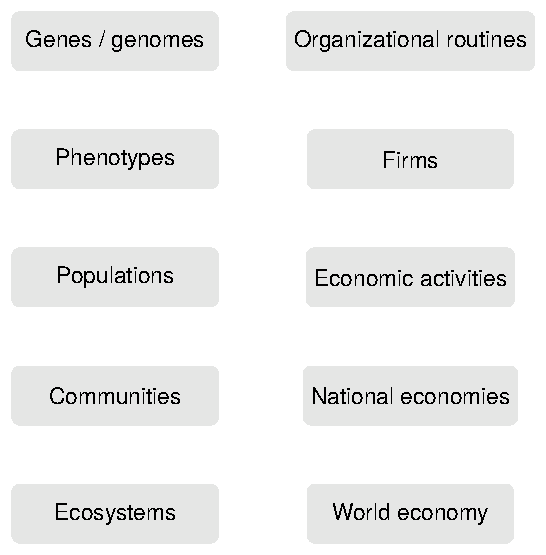
\includegraphics{organizational_complexity.pdf}
\caption{Schematic diagram of proposed organisational levels in biological and economic systems. \textbf{A} is inspired from \cite{Hendry+2016}}
\label{fig:organisational_levels}
\end{figure}

%% Figure micro / macro properties




\subsubsection*{Ecological and evolutionary processes drive the dynamics of biological systems}
% 
% History of the understanding of forces in ecology and evolution
% The challenge is to bridge the microscopic processes developing at a lower organizational level to deduce the long-term dynamics of these macroscopic features.
% % 
% The difficulty is to comprehend the coupling between the processes of interaction and evolution \cite{Strogatz2001a}. The former correspond to ecological processes, and involve fluxes of energy and matter across space and time, encompassing the processes of interaction between organisms (biotic interactions) and between organisms and their environment (abiotic interactions), and dispersal processes (movement of individual across space) \cite{Vellend2010a}. This term may also designate fluxes of information and capital between economic agents \cite{}.
%
% Biological systems are ruled by processes that have traditionally been grouped into two distinct classes, namely ecological and evolutionary processes \cite{Pelletier2009}.
% 
In biological systems, interaction processes are generally designated as ecological processes, and inolve fluxes of energy and matter across space and time, encompassing the processes of interaction between organisms (biotic interactions) and between organisms and their environment (abiotic interactions), and dispersal processes (movement of individual across space) \cite{Vellend2010a}.
% 
Evolutionary processes designate those processes responsible for the change of heritable characteristics (DNA, genes, phenotypes) over successive generations \cite{Hall2013}.
% 
The coupling between ecological and evolutionary processes is acknowledged since the very birth of the theory of Evolution, when Darwin realised a link between the different ecological opportunities across the Galápagos islands and the different beak shapes in the finches he found in each island \cite{darwin2004origin}, during his voyage on the Beagle.
% 
He reasoned that the variations in ecological opportunities lead to a differential in survival for certain phenotypes, which over time resulted in the evolution of different beak shapes.
% 
Since then, we know that ecological processes directly affect evolutionary response \cite{Ezard2009}.
% 
In the recent years, the idea that not only ecological processes can affect evolutionnary response, but also that evolutionnary processes could affect ecological processes, has developed \cite{XXX}.
% 
Empirical studies have demonstrated that evolution can be rapid and occur on similar time scales as ecology \cite{Hairston2005, Pelletier2009} and have quantifiable effects on ecological dynamics \cite{Ezard2009}, leading to feedbacks between ecological and evolutionary processes, so-called eco-evolutionary feedbacks \cite{Pelletier2009,Schoener2011}. 
% 
% Example of eco-evolutionary dynamics
Eco-evolutionary feedbacks involve situations where an ecological property influences evolutionary change, which then feeds back to an ecological property, or vice versa \cite{Govaert2019a}. Examples are feedbacks between population density (ecological property) and trait evolution (evolutionary change), which can lead to evolutionary branching through the effect of competition \cite{Doebeli1999}.
% 
Eco-evolutionary feedbacks are also involved in adaptation mechanisms \cite{Doebeli1999}, where species disperse and phenotypic variations allow to adapt to local environments \cite{XXX}.
% TODO: mention density dependence
% Empirically, \cite{XXX} shows that in the population of XX, XX happened.
% 
Those feedbacks may greatly influence the mechanisms driving the dynamics of ecosystems \cite{Urban2016}, but our understanding of their nature and effect is limited \cite{Lion2022}.
% 
In particular, eco-evolutionary feedbacks are expected to play a critical role in the evolution of the biosphere in the coming decades \cite{Norberg2012}, as ecosystems are being rapidly affected by anthropogenic pressure and with climate change \cite{Ellis2011,Midgley2019}.
% 
In order to mitigate the consequences of human development, it is of utmost urgency to better understand eco-evolutionary feedbacks \cite{Norberg2012}, and develop mechanistic models embedding this knowledge \cite{Urban2016}. This will in turn provide more reliable forecasts of ecosystem states \cite{Clark2001}, to help designing adequate management of ecosystem services \cite{Urban2016}.
% In particular, the answer to how species will adapt to increasing temperatures is uncertain due to our lack of understanding of eco-evolutionary feedbacks \cite{Norberg2012}. 
% 
% They are critically involved in adaptation mechanisms, which calls for 
%% Conclusion
% While eco-evolutionary feedbacks may greatly influence the mechanisms driving the dynamics of ecosystems \cite{Urban2016}, our quantitative understanding of their modality is limited \cite{Lion2022}. 
% 
% Beyond raising questions of sheer scientific interest, gaining such an understanding is a pressing need to mitigate the effect of global change.


\subsubsection*{Drivers of economic change}
The processes that determine economic change is controversial in economics \cite{Nelson2014}. 
%  This idiosyncrasy has been traditionally explained by geographic and institutional arguments \cite{C.A.HidalgoB.Klinger}. 
%% Mainstream econoomics vs evolutionary economics
To explain econonmic development, mainstream economic theory \cite{10.1093/cje/bet027} assumes that economic systems are in equilibrium, in the sense that the demand and supply of goods and services are balanced on all relevant markets. 
% TODO: Marks comments : transition from countries to firms is not quite clear to me here
Firms are rational in maximizing profits by adapting to demand and supply, and the observed economic change is driven by exogenous forces, such as technological change \cite{Romer1986}. Evolutionary economics, promoted by the seminal work of Ref. \cite{Nelson2014}, criticizes this view and seeks to explain economic change by focusing on endogenous forces. 
% 
%% Foundations of evolutionary economics
Evolutionary economics suggests that interactions between firms and economic activities, and evolutionary processes acting upon them, are major processes contributing to economic change \cite{Hodgson2019}.
% 
For instance, firms or economic activities may interact positively or negatively \cite{Wernerfelt1989,Pistorius2007Ozman2009,Saavedra2009a,Cohendet2018,Menon2015}, spread across space \cite{RogersEverettM2003DoI,Zahra2000}, and adapt \cite{Cordes2006} or transform into new econonmic institutions  \cite{Freeman2002,Hodgson2004,Aldrich2008}, affecting economic development at the regional and national scale.
%
%% biology as a way to understand economic dynamics
% Because such processes are analogous to the processes shaping the dynamics of biological populations and ecosystems, notorious economists such as Veblen \cite{Veblen1898} or Arrow \cite{doi:10.1126/science.267.5204.1617.g} have proposed that the appropriate paradigm to understand economic change should be evolutionary biology.
% 
% TODO: The processes of interaction and dispersal are analogous to ecological processes operating in biological systems \cite{XXX}, in that they also involve fluxes (of matter, information, and capital) between economic agents. By extension, we use eco-evolutionary processes and dynamics both in biological and economic systems.
% 
Because these processes are analogous to eco-evolutionary processes driving the dynamics of biological systems, a number of modelling approaches have borrowed concepts and methods from biology in the last decades, aiming at better understanding the processes underlying emergent properties in economic systems \cite{Tacchella2018,Saavedra2009a,Scholl2020,Zhang2018,Modis1997,Saavedra2014,Farmer1999,Michalakelis2011,Marasco2016,Gatabazi2019,Cauwels56,Applegate2021,Suweis2015}. 
% 
For instance, \cite{Saavedra2009a} has successfully used a model of mutualistic interaction to explain structural patterns in industrial cooperation.
% 
Also, \cite{Scholl2020} uses the concepts of foodwebs and density dependence to explain market malfunctions and excess volatility in financial markets.
% 
However, those studies did not seek to understand how these processes may affect economic development.
% 
Recent modelling approaches developed in evolutionary biology may help to disentangle whether eco-evolutionary processes could explain differences in economic development across countries.

\subsubsection*{Forward modelling of eco-evolutionary processes}
The complex interplay between ecological and evolutionary processes, acting at different scales of time and space and organization, can hardly be studied with experimental approaches \cite{Pontarp2019,Hagen2022}. 
% TODO: cite \cite{May2004}
As such, a deductive approach, relying on forward modelling, has traditionally been put forward to advance our understanding of the mechanisms underlying \cite{Brummitt2020}. Along this approach, hypotheses about causal processes are embedded in a model, wich forward integration generates emergent properties. Such emergent behavior may be seen as predictions from the consideration of the causal processes \cite{May2004}. The role of the modeller is to point at the mechanisms by which the properties emerge, disentangling the underlying interplay between the processes. % The resulting qualitative dynamics and/or quantitative predictions are validated against common intuition and empirical data, and further refined to elaborate a theory \cite{Sayama,Brummitt2020,Schmidt2009}.
% 
%% early mathematical models
In the early 1930s to 1940s, by formulating tractable mathematical models implementing the processes of reproduction, dispersal and mutations, the work of Fisher, Wright and Haldane has greatly contributed to the modern synthesis of evolutionary biology \cite{huxley1942evolution}, generally accepted as the basis of our current understanding of evolutionary dynamics. 
% 
The mechanistic models commonly take the form of differential equations (DE), and express how the processes under investigation affect the rate of change of the population characteristics, such as the proportion of a given allele. 
% 
However, the requirement of tractable mathematical models (DEs that yield analytical solutions) has involved strong assumptions on the processes investigated, that are poorly representative of the complexity of eco-evolutionary feedbacks in nature \cite{Govaert2019a}. In particular, ecological scenarios have been strongly simplified, and did not take into account how evolution could affect population dynamics \cite{Lion2022}. As such, traditional mathematical models have omitted eco-evolutionary feedbacks and density dependence.

%% computers
With the increase in computational capacity, novel modelling approaches relying on individual based models (IBMs) have appeared \cite{deangelis2005individual}. IBMs allow to capture processes acting at the individual level, requiring less simplifying assumptions than traditional mathematical models \cite{deangelis2005individual}. Capturing more realistic scenarios by allowing the forward integration of complex hypothesis, the lack of analytical tractability of IBMs may nonetheless occult the mechanisms underlying emergent properties \cite{Lion2016,May2004}.
% 
%% computers and analytical framework
The recent development of mathematical techniques, such moment closure approximations \cite{law1999moment,Gandhi2000,Nordbotten2020,Lion2016}, adaptive dynamics theory \cite{Metz1995}, and probability theory \cite{Champagnat2006}, are generating novel pathways by filling the gap between IBMs and mathematical models. 
% 
% They allow to derive analytical expressions for the population macroscopic properties (e.g., population size and trait variance) from individual-based assumptions. 
% 
Analogous to renormalisation group analysis developed in quantum and statistical physics \cite{Sayama}, they form a toolbox to rigorously derive how emergent properties are influenced by processes operating at different organizational levels. As such, they allow an analytical underpinning to IBM simulations, and can generate a general understanding of the key mechanisms at stake \cite{Lion2016}.

%% examples of the combination of computer models and analytical tools
The combination of numerical simulations and, e.g., adaptive dynamics theory, has successfully shed new lights on on the emergence of evolutionary branching under frequency-dependent selection \cite{Dieckmann1999,Doebeli2003}.
%
An other example is the work of \cite{Meszena1997,Debarre2013a, Mirrahimi2020}, that has provided new insights on the effect of habitat heterogenity on population dynamics. 
% 
However, our current understanding of eco-evolutionary feedbacks omits potentially significant factors, such as the structuration of populations over complex spatial structures \cite{XX} and highly dimensional phenotypic space \cite{XXX}.

% 
% For instance, the spatial scenario investigated in \cite{Gandon, Mirrahimi2016} merely involves two habitats, and it is unclear how their results would apply to more complex landscapes, such as mountains \cite{Rahbek2019}.
% 
The consideration of such details is important to advance our understadning, but raises challenging methodological issues. 
% 
In particular, complex models may hinder the fundament mechanisms underlying the emergence of a pattern.
% 
Also, the consideration of multiple traits leads to an increase in the dimensionality of the associated DE problem, which in turn leads to an exponential increase in computational cost \cite{XXX}.
% 
In order to better understand eco-evolutionary feedbacks, we need to investigate more realistic scenarios, which will, in turn, require the development of novel numerical methods that can cope with the extra computational cost.
% TODO: Marc;s comments: I like the last sentence that connects back to th eco-evolutionary modelling. It's a good introduction to the modelling approaches and well writen, but somehow I find it no so well connected to the problem. Maybe it's just because I don't fully understand :-)
% 
% This understanding uses matrices or networks to create representations of complex systems that do not ignore the identity of the elements involved or their interactions. These ideas, which are now prevalent in fields such as machine learning and physics, have begun to make their way into economics under the umbrella of economic complexity

\begin{figure}[t]
    \centering
    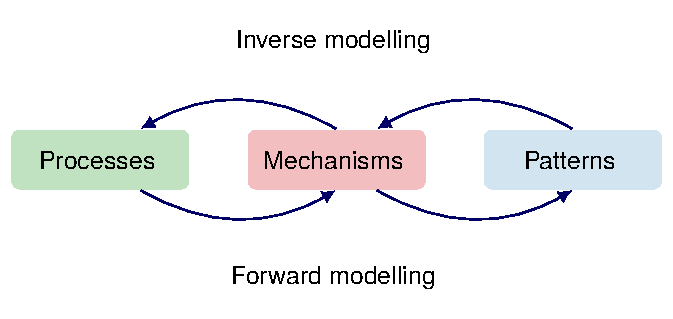
\includegraphics{proc_mech_patt.pdf}
    \caption{Forward and inverse modelling approaches for the understanding of CAS. A forward modelling approach starts with assuming a set of processes, and seeks to understand how their interplay transforms in mechanisms that are associated with macroscopic patterns. An inverse modelling approach starts from empirical patterns (or observations) to deduce the underlying mechanisms and associated processes.}
\end{figure}

\subsubsection*{Inverse modelling}
%% inverse modelling
While in forward modelling, observation data is uniquely considered at the end of the modelling cycle - when comparing predicted and empirical patterns to refine the baseline hypotheses -, inverse modelling integrates data at the start the modelling cycle \xxx (\cref{fig:forward_inverse_modelling}).
% 
% Diametrically opposed to forward modelling, inverse modelling consists in using observation data to infer causal processes \cite{Peng2011}. Inverse modelling has recently seen an increased attention, thanks to the increased computational power and availability of datasets \cite{Csillery2010}.
% 
%% Parameter estimation
Inverse modelling can take the form of parameter estimation \cite{Schartau2017} or model selection \cite{Johnson2004}, both involving the use of inference methods to estimate, respectively, the most probable model parameter value, or the most probable model among candidates, given the data.
% 
% involves the use of inference methods to estimate the most probable model parameter value given the data \cite{Schartau2017}. They can also be used to test the support of competing hypotheses, embedded in alternative models, where 
% 
% such as bayesian or maximum likelihood inference methods . 
% 
% Those methods proceed by defining a distance between the model simulation and the observation data, which relates to the probability of the parameters given the model and the data \cite{Schartau2017}. The most likely parameters are associated with the minimum distance, obtained using ad-hoc algorithms.
% 
Provided that they are inferred together with uncertainties, parameters can be interpreted to better understand the strengths and effects of the associated processes \cite{Pontarp2019}. For instance, \cite{Higgins2010,Curtsdotter2019} infer and analyse the parameters of population dynamic models to understand processes involved in ecosystem functions.
%
In model selection, the candidate models embed competing hypotheses about processes and mechanisms, and the relative support of each model given the data is used to discriminate \cite{Johnson2004}. For instance, \cite{Skeels2022} shows that temperature-dependent evolutionary speed is the most likely mechanism to explain variations in biodiversity patterns, using inference methods to discriminate between alternative dynamic models embedding different evolutionary hypotheses.
% 
The inference methods used to calculate the parameter and model probabilities proceed by defining a distance between the model simulation and the observation data \xxx, which relates to the probability of the parameters given the model and the data \cite{Schartau2017}. In parameter estimation, the most likely parameters are associated with the minimum distance to the data \xxx, and in model selection, the most likely models are associated with the minimum of the minimum model distance \xxx.
% 
Inference methods involve numerical methods to recover the model distance to the data \xxx, which success is dependent on the model formulation and its dynamical properties \xxx.
% 
% The parameter estimation problem consists in finding the maximum probability of the model given the observation data, inference methods can also be used to discriminate between candidate mechanisms embedded in alternative models \cite{Burnham2002,Johnson2004}. For instance, \cite{Skeels2022} shows that temperature-dependent evolutionary speed is the most likely mechanism to explain variations in biodiversity patterns, using inference methods to discriminate between alternative dynamic models embedding different hypotheses.
% 
% For instance, \cite{Higgins2010,Curtsdotter2019} infers and analyse the parameters of population dynamic models to understand processes involved in ecosystem functions.
% 
Thus far, the use of inverse modelling for understanding eco-evolutionary dynamics has been limited because of a number of issues, including the high computational cost of the forward integration of eco-evolutionary models \cite{Fisher2018}, the large number of parameters involved \cite{Boyd2012}, and their strong nonlinearities \cite{Hastings1993,Huisman1999,Beninca2008}. Advances in the field of artificial intelligence could circumvent these issues, allowin to confront eco-evolutionary models with data \xxx.

\subsubsection*{Machine learning to leverage forward and inverse modelling}

In the recent years, the field of artificial intelligence (AI) has made enormous progresses in computer vision \cite{XXX} and natural language processing \cite{XXX}. At the backbone of this success are key computational techniques that could leverage the forward and inverse modelling of CAS.
% 
% AI uses observation data to learn abstraction of mechanisms and make prediction about the world, 
% 
%% AI and neural networks
% 
% Neural networks are universal approximators \cite{XXX}, i.e. parametric functions that can theoretical approximate any high dimensional function, such as the function that allows us to differentiate a cat from a dog.
% 
% Neural networks are computational models with very good properties to interpolate data \cite{xxx}, and have been used, for instance, to build species distribution models from occurrence datasets \cite{Deneu2021}.
% 
Computer vision and natural language processing rely on deep learning methods, that allow neural networks to learn abstract representation of mechanisms from large datasets \cite{LeCun2015}.
% 
These abstractions are hardly interpretable by humans \cite{XXX}, and their prediction ability is limited by the information contained in the training datasets. As such, neural networks cannot be used \textit{per se} to gain scientific insights and extrapolate beyond observed trends \cite{Barnosky2012,Urban2016}. %Last but not least, the success of the learning process in tightly linked to the quantity of data available for training. Yet in many scientific domains -- comprising evolutionary biology and economics -- the expense, or impossibility, of conducting experiments prohibits the collection of large datasets.
% 
Nevertheless, their traditional applications and associated methods have been successfully derived in other scientific fields for this purpose \cite{Kashinath2021,Schneider2017,Yazdani2020,Rolnick2023}.

%
%% ML for forward modelling
Neural networks have been used in forward modelling, to reduce the cost of the forward integration of climate models, by learning more efficient representations of physical mechanisms \cite{XXX}.
% 
They have also been used to approximate the solution of partial differential equations (PDEs) \cite{sirignano2018dgm}, with the major advantage of approximating high dimensional problems at a lower computational cost than traditional methods.
% 
% Notoriously, \cite{Arnulf} has developed methods consisting in training neural networks through a correspondence between PDEs and stochastic processes. \cite{Arnulf} have mathematically proved and numerically showed that their methods can efficiently approximate very high dimensional PDEs (10 000 dimensions), which could allow to include more realism in eco-evolutionary models.
% 
% Nonetheless, PDE models for CAS critically involve non-local terms, which capture non-local interactions between microscopic agents. The extension of such techniques to non-local PDEs could leverage the forward modelling of biological and economic systems.
%
%% ML for inverse modelling
% Neural networks have also been employed to leverage inverse modelling techniques.
% 
Underlying the training of neural network is the technique of backpropgation \cite{XXX}. This technique can be generalised to any scientific model against data \cite{Rackauckas2020}, with the potential to leverage inverse modelling techniques. %With the ability to handle computational models characterised by a very large number of parameters, AD, together with the development of other training techniques \cite{XXX}, have the potential to leverage inverse modelling \cite{Rackauckas2020}.
% 
% For instance, automatic differentiation has allowed symbolic regression, automatically generating symbolic equations for nonlinear coupled dynamical systems directly from time series data \cite{WOS:000247363000007}. Cons: this method is "model-free", and is rather more relevant in engineering. It generates equation from a bank of polynomials, but is not suited for testing a bunch of different models. It also handle model with simple dynamics, while real-world systems often show chaotic dynamics. Identifying only the useful analytical relations that are related to the system dynamics. still faced with the challenge of justifying and giving words to their meaning. One difficulty is that we cannot know with certainty the units of bulk constants in the law ex- pressions (for example, combinations of masses, lengths, etc. embodied in the system). Second, the equation may model something that is inherently difficult to observe directly, such as total energy. Requiring equations to maintain consistent physical units still leaves room for ambiguity. \cite{Schmidt2009} \cite{Mangan2017}.
% 
As such, the derivation of AI techniques to investigate causal processes in CAS offers unique opportunities \cite{Frank2022}.

% to be checked tomorrow (01/09)
% Recent advances in interpretable ML are enbling the generation of theories to be automated. Mathematical laws, that took many years for scientists to solve manually, have been identified in physical and biological systems.

% the abstractions that they learn from the data is inscrutable
% This learning process is allowed by using the backpropgation algorithm, to indicate how a machine should change its internal 

% The predictive ability of mechanistic models has remained poor \cite{DeAngelis2015}, due to a low pervasion of observation data in mechanistic models \cite{XXX}.

\subsubsection*{Programming languages}

Combining ML techniques with scientific models requires computational environments that allow to easily develop scientific models, ensure simulation performance, and provide composability between ML and other scientific libraries \cite{Rackauckas2020}. Unfortunately, performance and composability are features that are poorly represented in mainstream programming languages used by the scientific community, such as Python, Matlab or R.
% 
%% performance and ease of use
Those languages are naturally attractive because they are dynamically typed \cite{XX}, allowing convenient development iterations. Nonetheless, prototypes written in Python, Matlab or R need to be rewritten in low level, compiled languages such as C, C++ or Fortran for speed and predictable mapping to hardware \cite{Perkel2019,Bezanson2017}. This conversion requires significant involvement, leading to a problem commonly designated as the "two language problem" \cite{Bezanson2017}.
% 
In order to circumvent issues of performance, most libraries in Python, Matlab or R rely on bindings with low level languages. For instance, the most used deep learning libraries in Python, TensorFlow and PyTorch, are internally written in C. However, bindings with low level languages come with major negative externalities, such as restricting the understandability of their internals to computer scientists -- prohibiting potential development contributions from the scientific community --, and preventing the composability of libraries \cite{XXX}. 

%% Julia 
Julia is a programming language that was launched in 2012 to address the issue of the two-language problem \cite{Bezanson2017,Bezanson2018}. Julia was built over a type-specializing, just-in-time compiler, which makes it easy to generate highly performant programs, while preserving the essential features of Python, Matlab or R, such as dynamic typing and automatic memory management.
% 
Importantly, it relies on multiple dispatch, which allows to generate highly generic code with good performance. This permits to write libraries in pure Julia, guaranteeing productivity and composability.
% 
% In particular, multiple dispatch allows users to build functions that, without containing a single code of GPU-specific code, can be automatically compiled to work on GPUs, using custom types \cite{GPUArrays.jl}. 
% 
As such, the internals of any Julia library can be understood by non computer-scientis, who can further use his expertise to participate to its development. Many Julia libraries benefit from a high number of contributions of independent users (see, e.g., \href{github.com/DifferentialEquations.jl}{github.com/DifferentialEquations.jl}).
% 
Multiple dispatch also allows to automatically generate the gradient of any Julia program without any modification \cite{ForwardDiff.jl, Zygote.jl}. This means that any scientific library in Julia, such as differential equation solvers, can be combined with deep learning tools, with unique opportunities for forward and inverse modelling problems \cite{Frank2022}. 
% 
% This unique feature has motivated the Climate Modelling Alliance to build an entirely new climate model in Julia, in order to obtain compatibility with ML libraries with the aim of improving predictions with data \cite{Tapio}.
% 
As such, Julia allows to prototype a program which is readily generic and can directly be shared to the research community. Further, by granting the composability of libraries, it allows to blend ML techniques with scientific models. This makes Julia a promising computational environment to accelerate research in CAS. 

\subsubsection*{Thesis outline}

In summary, while it is increasingly acknowledged that feedbacks between ecological and evolutionary processes play an important role in the dynamics of biological systems \cite{Pelletier2009, Urban2016}, our understanding of the mechanisms in which they are involved has been limited to simplified scenarios.
% 
Further, while analogous processes have been suggested to influence the dynamics of economic systems \cite{Hodgson2019}, a quantification of their effect is missing.
%
Under increasing anthropogenic pressure, these research directions become essential \cite{Urban2016}, but raise challenging methodological issues.
% 
Here, I present novel forward and inverse modelling approaches to advance our understanding of eco-evolutionary dynamics in biological and economic systems, and utilise them to shed light on the underlying processes and resulting mechanisms.


In \cref{chap:diff-in-graphs}, I investigate how eco-evolutionary processes, in combination with complex habitat spatial structures, influence the trait distribution of biological populations. 
I proceed using a forward modelling approach, building a stochastic eco-evolutionary IBM where individuals are structured over a spatial graph, and experience the fundamental processes of reproduction, competition, mutation and migration. I seek to understand how those microscopic forces result in trait differentiation at the population level. I derive DE approximations of the IBM that, together with extensive numerical simulations, provide analytical insights into how the graph properties affect the population size and trait differentiation. In particular, I show that three main graph properties, measuring landscape connectivity, heterogeneity in connectivity, and habitat spatial auto-correlation, shape the trait differentiation of the biological population. These results establish mechanistic links between landscape features and the eco-evolutionary dynamics of biological populations.

In \cref{chap:mini-batching}, I develop an inverse modelling method to estimate the parameters of highly nonlinear population dynamic models. The method is based on a machine learning framework and involves AI techniques together with a novel learning strategy. This learning strategy consists in training the model against mini-batches of data with short time horizon, which I analytically show to regularize the learning problem. I implement the ML framework in the Julia library \textbf{MiniBatchInference.jl}, and demonstrate through numerical experiments that it can efficiently estimate model parameters and provide statistical evidences for causal processes from noisy, incomplete and independent time series. Altogether, the proposed ML framework is a workhorse for inverse modelling and can elucidate mechanistic pathways in biological and economic systems.

In \cref{chap:econobiology}, I quantify the effect of eco-evolutionary processes on the dynamics of economic systems. I employ the ML framework developed in \cref{chap:mini-batching} to investigate how alternative eco-evolutionary population dynamic models can explain the dynamics of economic activities in the richest 100 countries, relying on 59 year of economic data. The models embed the processes of ecological interactions between economic activities, spatial transfers, and economic activity transformations, which support is compared to a simple logistic growth model, taken as a null model. I find strong statistical evidence for positive interactions between national economic activities, and spatial transfers across countries. To my knowledge, this is the first study that provides quantitative evidences that similar processes may influence the dynamics of biological and economic systems.

In \cref{chap:non-localPDE}, I extend two recent methods to solve high dimensional PDEs, in order to handle non-local nonlinear terms. The first method relies on Picard iterations, while the second is based on machine learning and involves neural networks to approximate PDE solutions. The numerical difficulties arising due to the non-local term are avoided by using a plain vanilla Monte Carlo integration. I implement the methods in the Julia library \textbf{HighDimPDE.jl}, and evaluate their performance on high dimensional PDE models arising in physics and biology, including population dynamic eco-evolutionary models. For all models, the methods yield good results with short run times, offering the possibility to include more realism in future eco-evolutionary models.

\newpage

% remains to be understood, and is more important than ever in a rapidly changing world.

% \section{Complex adaptive systems}
% \label{sec:intro:cas}
% \begin{outline}
%     \1 A central aim in the discipline of Ecology is to determin the underlying causes of variation in the abundance and sitribution of species.
%     \1 Ecological and economic systems are complex adaptive systems (CAS): they are systems that are composed of many entities with heterogeneous characteristics, which interact and experience selection processes. Those processes act at the individual level, but are key in determining the macroscopic behaviour at the system level, a feature that make those systems unique.
%     \1 Complex interconnected systems pose a major challeng to scientific study in ecology and economics \cite{Ye2016} (and references therin).
%         \2 the common approach of reducing these systems to linearly independent components overlooks important interactions for the sake of computational tractability 
%         \2 statistical frameworks (e.g., PCA, GLM, multivariate autoregressive models), assume that caysal factors do not interact with each other and have independent or additive effects on a response variable,
%             \3 simplification leads to probelms in identifying associations (refs 5-6 of \cite{Ye2016})
%             \3 cannot predict out-of sample behaviour
%         \2 complex equation-based modeol explicitly accounting for each interaction have great intuitive appeal 
%             \3 but those models suffer from their many parameters to be precisely determined given the available data (curse of dimensionality (ref 9 \cite{Ye2016}))
%             \3 problem is amplified because in biological fields the relevant units may not behave according to the fundamental equations.
% \end{outline}
% \subsubsection{Biological systems}
% \begin{outline}
%     \1 Biodiversity results from a hierarchy of processes acting at different scales of time and space. Variations experienced by organisms, their interactions between them and with the environment, and selection pressure acting upon groups of organisms are of particular relevance for explaining differences in species richness at the ecosystem levels.
%             \2 The synthetic  theory of evolution (see e.g. Gayon 2003): with genetics (Mendel) and DNA (James Watson and Francis Crick)
%             \2 \textit{Nothing in biology makes sense except in the light of evolution} (Dobhansky 1973)
%     \1 explanation for the main principles underlying the emergence of biodiversity: mutliple processes that interact at different scale in space and time 
%             \2 allopatric speciation
%             \2 ecological speciation 
%             \2 dispersal
%             \2 adaptation
%             \2 those processes interact simulatneously withing the surrounding environment
%     \1 Traits: measurable characteristics that reflect and shape evolutionary history (Darwin 1859). Natural selection promotes the evolution of traits thatoptimize species survival under specific environmental conditions..
% \end{outline}
% \subsubsection{Economic systems}
% \begin{outline}
%     \1 The economic trajectory of a country is greatly affected by the ensemble of economic actors and their interactions, that structure its economy. Firms are adaptive entities that respond to the environment in which they operate according to their characteristics, that vary over time. By interacting together and experiencing selection pressure, they determine economic growth at the country level.
%         \2 \textbf{Universal Darwinism}
% \end{outline}
% \subsubsection{Research questions}
% \begin{outline}
%     \1 Despite the intrinsic variability of the entities that compose them, and despite the complexity of the processes driving their dynamics, regularities at the macroscopic level emerge in ecological and economic systems. This is the case of large-scale spatial patterns of biodiversity and differences in economic growth across countries, calling for a mechanistic understanding of the essential mechanisms that generate them.
%         \2 Multiple arrangements of parts that result in a complex set of effects in a system are defined as mechanisms (Dawkins 2010)
% \end{outline}

% \section{Eco evolutionary processes}
% \begin{outline}
%     \1 Eco-evolutionary processes and analogous economic processes acting upon firms have been proposed to play a major role in the emergence of macroscopic patterns in ecological and economic systems. Nonetheless, a quantitative investigation of their importance is missing.
%         \2 The interplay between ecological processes, the processes that regulate interactions between organisms, and evolutionary processes, the change of the characteristics of biological populations over time, has recently received increasing attention to explain current biodiversity patterns. 
%         \2 Analogous economic processes have been proposed to explain differences in economic growth across nations.
%     \1 A quantitative investigation of how those patterns can emerge from eco-evolutionary processes is required to improve our current understanding and generate a parsimonious theory with predictive power. This defines the goal of this project, which undertakes this investigation through a unique approach that consists in confronting quantitative eco-evolutionary models to empirical data.
% \end{outline}

% \section{Models and challenges}
% \begin{outline}
%     \1 Eco-evolutionary models are complicated and necessitate the use of computers to be simulated and analysed against data. This poses a number of methodological challenges that we adress in the first part of this project.
%         \2 Entities in CAS have distinct quantitative attributes that determine their fitness in a given environment. Accounting for the variety of these characteristics leads to models with high dimensionality, associated to a high if not prohibitive computational cost preventing its simulation.
%             \3 The model zoo
%                 \4 Agent Based model: hard to scale up
%                 \4 PDE: hard to scale up
%                 \4 In particular, partial differential equation (PDE) models, which can encode eco-evolutionary processes acting upon entities defined by many characteristics, are cursed by their dimensionality.
%                 \4 Machine learning: scale up
%             \3 To this aim, we develop machine learning algorithms that break down the curse of dimensionality by relying on neural networks to approximate the solution to PDE models.
%         \2 An other difficulty consists in confronting eco-evolutionary models with data, since those models cannot be manipulated by standard statistical techniques. 
%             \3 We apply methods commonly employed in the training of neural networks, together with model selection techniques, to infer from candidate models fundamental mechanisms that characterise the patterns under investigation.
%     \1 The machine learning approximations that we develop allow for efficient model simulations, that we combine with training techniques and model selection methods to explore the motivated research question.
% \end{outline}

% \missingfigure{Here you could add a coneptual figure, similar to Florian Patout (see evernote), that shows the interplay between selection and variation.}

% \section{Machine learning : opportuntities}
% \begin{outline}
%     \1 State of the art machine learning techniques have yielded transformative results across divers scientific disciplines [REF], but rely on a large amount of data [REF], while environmental sciences rely in a small data regime where those techniques are typically not suited \cite{Raissi2019a}. Recently, physics informed machine learning has emerged as a tool to constrain fully parametric methods with scientific knowledge, for data efficiency and extrapolation \cite{Raissi2019a}. The key idea is to refine the learning with scientific knowledge by adding additional constraints in the objective function, given by ODEs/ PDEs models.
%     \1 \cite{Karpatne2017}
%     \1 \cite{Rolnick2023}, Tackling Climate Change with Machine Learning: Changes in climate are increasingly affecting the distribution and composition ofecosystems. This has profound implications for global biodiversity, as well as agriculture, disease, and natural re- sources such as wood and fish. ML can help by supporting efforts to monitor ecosystems and biodiversity.
%     Monitoring
% \end{outline}

% \section{Learning from models}
% \begin{outline}
%     \1 we develop quantitative models that embed general eco-evolutionary processes, and test them against data to explore hypotheses on the fundamental mechanisms that drive patterns of biodiversity and economic growth.
%         \2 From one hand, we explore how eco-evolutionary processes, in combination with complex landscape topologies, can explain patterns of species diversity.
%         \2 To this aim, we develop and analyse an eco-evolutionary model on spatial graphs, to understand how the combination of eco-evolutionary processes and complex landscapes might have shaped biodiversity patterns that are found in complex landscapes such as mountain regions.
%         \2 On the other hand, we investigate how eco-evolutionary processes can provide new insights in the understanding of economic dynamics.
%         \2 We proceed by developing a simple eco-evolutionary model which explanatory power we test against long time series that capture the dynamics of asset size of economic sectors.
%     \1 Overall, this project is a step towards providing a useful conceptualisation of fundamental eco-evolutionary mechanisms that shape the features of the world that surrounds us.
% \end{outline}


% \section{Thesis outline}
% \label{sec:intro:structure}

% \textbf{Part \ref{part:I}\\
% An eco-evolutionary model on spatial graphs} \\[0.2em]
% It is not clear how landscape connectivity and habitat heterogeneity influence differentiation in biological populations. 
% %
% To obtain a mechanistic understanding of underlying processes, we construct an individual-based model that accounts for eco-evolutionary and spatial dynamics over graphs. 
% %
% Individuals possess both neutral and adaptive traits, whose co-evolution results in differentiation at the population level.
% %
% In agreement with empirical studies, we show that characteristic length, heterogeneity in degree and habitat assortativity drive differentiation.
% %
% By using analytical tools that permit a macroscopic description of the dynamics, we further link differentiation patterns to the mechanisms that generate them.
% %
% This part provides support for a mechanistic understanding of how landscape features affect diversification.

% \textbf{Part \ref{part:II}\\
% Scientific machine learning for eco-evolutionary modelling} \\[0.2em]
% % Mechanistic models crystallise hypothesis into a synthetic framework that allows for a description of mechanisms driving the dynamics of complex adaptive systems.
% %
% It is a daunting task to obtain an agreement between mechanistic models and real world systems. In particular, there is a need to account for the dimensionality of the evolutionary and spatial structures over which agents interact and evolve. Furthermore, the calibration of such models is difficult.
% % given that direct measurements to estimate quantities of interest are in general not possible, and only a small set of undirect observations are available.
% %
% To adress the difficulties that arise due to the dimensionality of models, we develop two numerical methods to solve high-dimensional non-local nonlinear PDES that arise in eco-evolutionary models. We implement those methods in a software, \texttt{HighDimPDE.jl}, that integrates within an open source ecosystem for Scientific Machine Learning in the Julia programming language.
% %
% We further present a scheme to estimate the parameters of a mechanistic model from empirical data sets. We show with analytical arguments that the use of different shallow time series allows for a better estimation than a unique, possibly deeper time series.
% %
% This part provides ready-to-use modeling tools to adress the intrinsic complexity of complex adaptive systems.

% \textbf{Part \ref{part:III}\\
% Briding eco-evolutionary models and data} \\[0.2em]
% Despite evidences that alike biological systems, economic systems are complex adaptive systems that continuously adapt and experience evolutionary processes, economists have discarded biological models and have rather relied on mechanistic models inspired from physics.
% %
% Building upon an analogy between economic sectors and biological functional groups, we use a biological model to quantitatively investigate whether eco-evolutionary processes characterise the dynamics of economic sectors.
% %
% Overall, we find that interactions across economic sectors, evolution of new economic sectors, and international transfers play a major role in the dynamics of economic sectors at the national level. 
% %
% The significance and the strength of such processes strongly vary across countries and correlate with standard macroeconomic indices such as the Economic Complexity Index.
% %
% We relate such patterns to documented patterns in ecology and evolution.
% %
% This part provides a new perspective on the understanding of the dynamics of economic systems.
% % 
% % The mechanistic framework is inspired from theoreteical biology that is general enough to encompass forces and processes in both economics systems and ecological systems


% \begin{comment}
%     The text of this thesis/dissertation contains reprints of the material as it appears in journals.
% \end{comment}

\printbibliography[heading=subbibliography]